%\documentclass{beamer}
%\usepackage{minijs}
%\usepackage{here}
%\mode<presentation>{
%  \usetheme{Antibes}
%  \usecolortheme{beaver}
%  \setbeamercovered{transparent}
%}
\documentclass[13pt,dvipdfmx]{beamer}
\usepackage[english]{babel}
% pdfの栞の字化けを防ぐ
\AtBeginDvi{\special{pdf:tounicode EUC-UCS2}}
% テーマ
\usetheme{CambridgeUS}
\usecolortheme{dolphin}
\usepackage{caption}
\setbeamertemplate{navigation symbols}{} 
\usepackage{graphicx}
\usepackage{amsmath}
\usepackage{amssymb}
\usepackage{txfonts}
\usepackage{colortbl}
\usepackage{svg}
\usepackage{pdfpages}
\renewcommand{\familydefault}{\sfdefault}
\renewcommand{\kanjifamilydefault}{\gtdefault}
\setbeamerfont{title}{size=\large,series=\bfseries}
\setbeamerfont{frametitle}{size=\large,series=\bfseries}
\setbeamertemplate{frametitle}[default][center]
\usefonttheme{professionalfonts}

%1ページめ
\title[クラスタリング手法の評価]{クラスタサイズ調整変数を導入したクラスタリング手法の評価}
\author{池辺 颯一}
\institute[情報数理工学研究室]{情報数理工学研究室 \and af16009@shibaura-it.ac.jp}
\date{2019年1月16日}

\begin{document}
\begin{frame}\frametitle{}
  \titlepage
\end{frame}

\section{導入}
\begin{frame}\frametitle{研究背景}
 \begin{block}{クラスタリング}
  \begin{itemize}
   \item 情報通信社会の発展に伴いデータ量が増大
   \item データを類似度に基づきグループ化するクラスタリングに着目
  \end{itemize}
 \end{block}
 \begin{block}{クラスタリングの欠点}
  \begin{itemize}
   \item 各クラスタのサイズに差がある場合に有意な結果が得られない場合がある
   \item クラスタのサイズを考慮して分類をする手法が提案されている
  \end{itemize}
 \end{block}
\end{frame}

\begin{frame}\frametitle{研究目的}
  \begin{block}{目的}
   クラスタサイズ調整変数を導入した手法について
   \begin{itemize}
    \item 各手法の特性を把握
    \item 最も有用なものを発見
   \end{itemize}
  \end{block}
  \vspace{4mm}
  \begin{block}{目標}
    \begin{itemize}
    \item 各手法で2クラス分類を行い特性を把握する
    \item 各手法のクラスタリング精度の算出及び比較を行う
   \end{itemize}
  \end{block}
\end{frame}

\begin{frame}\frametitle{実験対象}
  \begin{block}{提案手法}
    \begin{itemize}
    \item eFCMA
    \item qFCMA
    \item sFCMA
    \end{itemize}
  \end{block}
\end{frame}

\begin{frame}\frametitle{クラスタリングの最適化問題}
  \begin{block}{eFCMA}
    \quad$\underset{u,v,\alpha}{\text{minimize}}$
    $\sum_{i=1}^C\sum_{k=1}^Nu_{i,k}||x_k-v_i||_2^2+\lambda^{-1}\sum_{i=1}^C\sum_{k=1}^Nu_{i,k}\log\Bigl(\frac{u_{i,k}}{\alpha_{i}}\Bigl)$\\
    \qquad\qquad\qquad\quad{\text{subject to }}$\sum_{i=1}^Cu_{i,k}=1$\;,\;$\sum_{i=1}^C\alpha_{i}=1$\;and\;$\lambda>0,$\quad$\alpha_{i}>0$
  \end{block}
  \begin{center}
    \begin{tabular}{c|c||c|c} \hline
	  {$N$}&データ数&{$x_k$}&データ数 \\ \hline
	  {$C$}&クラスタ数&{$v_i$}&クラスタ中心\\ \hline
	  {$\lambda$}&ファジィ化パラメータ&{$u_{i,k}$}&帰属度 \\ \hline
	  {$\alpha_i$}&クラスタサイズ調整変数\\ \hline
    \end{tabular}
  \end{center}
\end{frame}

\begin{frame}\frametitle{クラスタリングの最適化問題}
  \begin{block}{qFCMA}
    \quad$\underset{u,v,\alpha}{\text{minimize}}$
    $\sum_{i=1}^C\sum_{k=1}^N(\alpha_{i})^{1-m}(u_{i,k})^m||x_k-v_i||_2^2$
    $+\frac{\lambda^{-1}}{m-1}\sum_{i=1}^C\sum_{k=1}^N(\alpha_{i})^{1-m}(u_{i,k})^m$\\
    \qquad\qquad{\text{subject to }}$\sum_{i=1}^Cu_{i,k}=1$\;, \;$\sum_{i=1}^C\alpha_{i}=1$\; and \;$\lambda>0$\;, \;$m>1$\;, \;$\alpha_{i}>0$
  \end{block}
  \begin{center}
    \begin{tabular}{c|c||c|c} \hline
	  {$N$}&データ数&{$x_k$}&データ数 \\ \hline
	  {$C$}&クラスタ数&{$v_i$}&クラスタ中心\\ \hline
	  {$\lambda,m$}&ファジィ化パラメータ&{$u_{i,k}$}&帰属度 \\ \hline
	  {$\alpha_i$}&クラスタサイズ調整変数\\ \hline
    \end{tabular}
  \end{center}
\end{frame}

\begin{frame}\frametitle{クラスタリングの最適化問題}
  \begin{block}{sFCMA}
    \quad$\underset{u,v,\alpha}{\text{minimize}}$
    $\sum_{i=1}^C\sum_{k=1}^N(\alpha_{i})^{1-m}(u_{i,k})^m||x_k-v_i||_2^2$\\
    \qquad\qquad\quad{\text{subject to }}$\sum_{i=1}^Cu_{i,k}=1$\;, \;$\sum_{i=1}^C\alpha_{i}=1$\; and \;$m>1$\;, \;$\alpha_{i}>0$
  \end{block}
  \begin{center}
    \begin{tabular}{c|c||c|c} \hline
	  {$N$}&データ数&{$x_k$}&データ数 \\ \hline
	  {$C$}&クラスタ数&{$v_i$}&クラスタ中心\\ \hline
	  {$m$}&ファジィ化パラメータ&{$u_{i,k}$}&帰属度 \\ \hline
	  {$\alpha_i$}&クラスタサイズ調整変数\\ \hline
    \end{tabular}
  \end{center}
\end{frame}

\begin{frame}\frametitle{研究方法}
 \begin{block}{研究手順}
   \begin{enumerate}
    \item 人工データ実験
    \item 実データ実験
    \item 実データ実験で算出したARIにより各手法を評価
    \item 3手法の中でARIの最高値が算出された手法を高評価とする
   \end{enumerate}
  \end{block}
\end{frame}

\begin{frame}\frametitle{研究方法}
 \begin{block}{人工データ実験の評価指標}
  \begin{itemize}
   \item 評価指標として分類関数を用いる
  \end{itemize}
 \end{block}
 \begin{block}{実データ実験の評価指標}
  \begin{itemize}
   \item 評価指標としてARI(Adjusted Rand Index)を用いる
   \item $-1$から$1$までの範囲で精度評価を行う指標
   \item $1$の時に完全一致で$0$の時にランダム
   \item ARIの値が高いほど高評価
  \end{itemize}
 \end{block}
\end{frame}


\section{人工データ実験}
\begin{frame}\frametitle{人工データ実験}
  \begin{block}{使用する人工データ}
    \begin{itemize}
    \item 平均値($-1$, $-1$), 標準偏差($0.5$, $0.5$)及び平均値($1$, $1$), 標準偏差($0.5$, $0.5$)のガウスサンプリングで生成
    \item データ数: $100$
    \item クラス数 : $2$
    \end{itemize}
    \begin{center}
     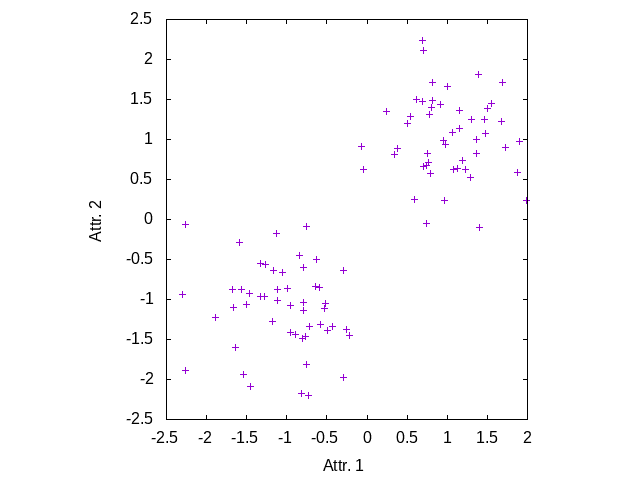
\includegraphics[width=60mm]{2d-dat.png}
    \end{center}
  \end{block}
\end{frame}

\begin{frame}\frametitle{アルゴリズム}
  \begin{enumerate}
  \item クラスタ中心をランダムに与える.
  \item クラスタ中心を用いて帰属度を更新する.
  \item 帰属度を用いてクラスタ中心及びクラスタサイズ調整変数を更新する.
  \item 収束すれば終了し,そうでない場合は$2$に戻る.
  \end{enumerate}
\end{frame}

\begin{frame}\frametitle{実験結果}
  \begin{block}{eFCMA}
    \begin{figure}[htbp]
      \begin{minipage}{0.32\hsize}
        \begin{center}
          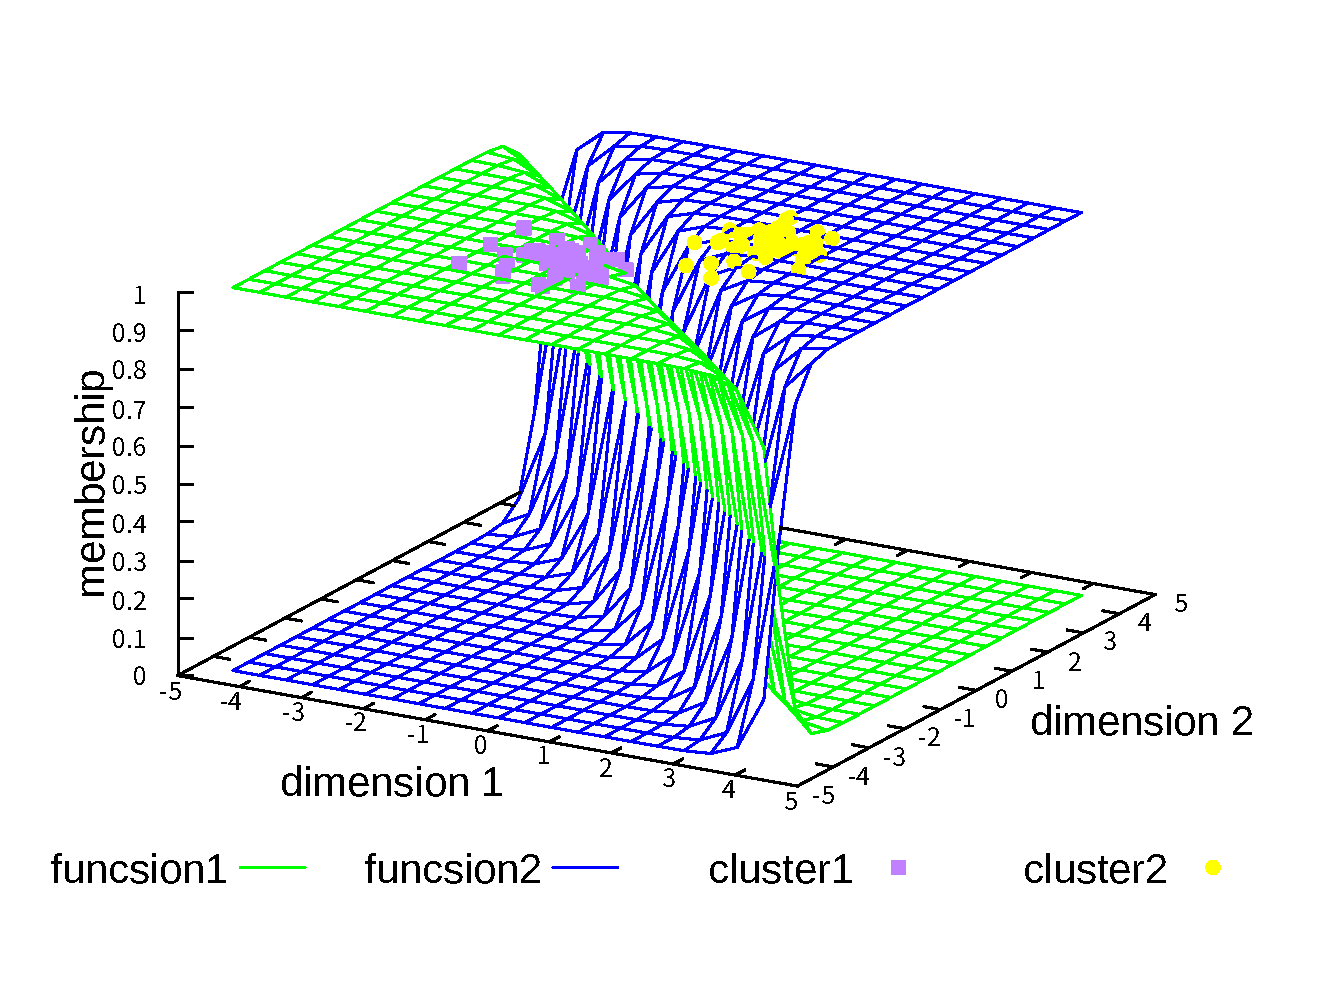
\includegraphics[width=40mm]{eFCMA-Lambda1.pdf}
        \end{center}
        \captionsetup{labelformat=empty,labelsep=none}
        \caption{$\lambda=1$}
        \label{fig:one}
      \end{minipage}
      \begin{minipage}{0.32\hsize}
        \begin{center}
          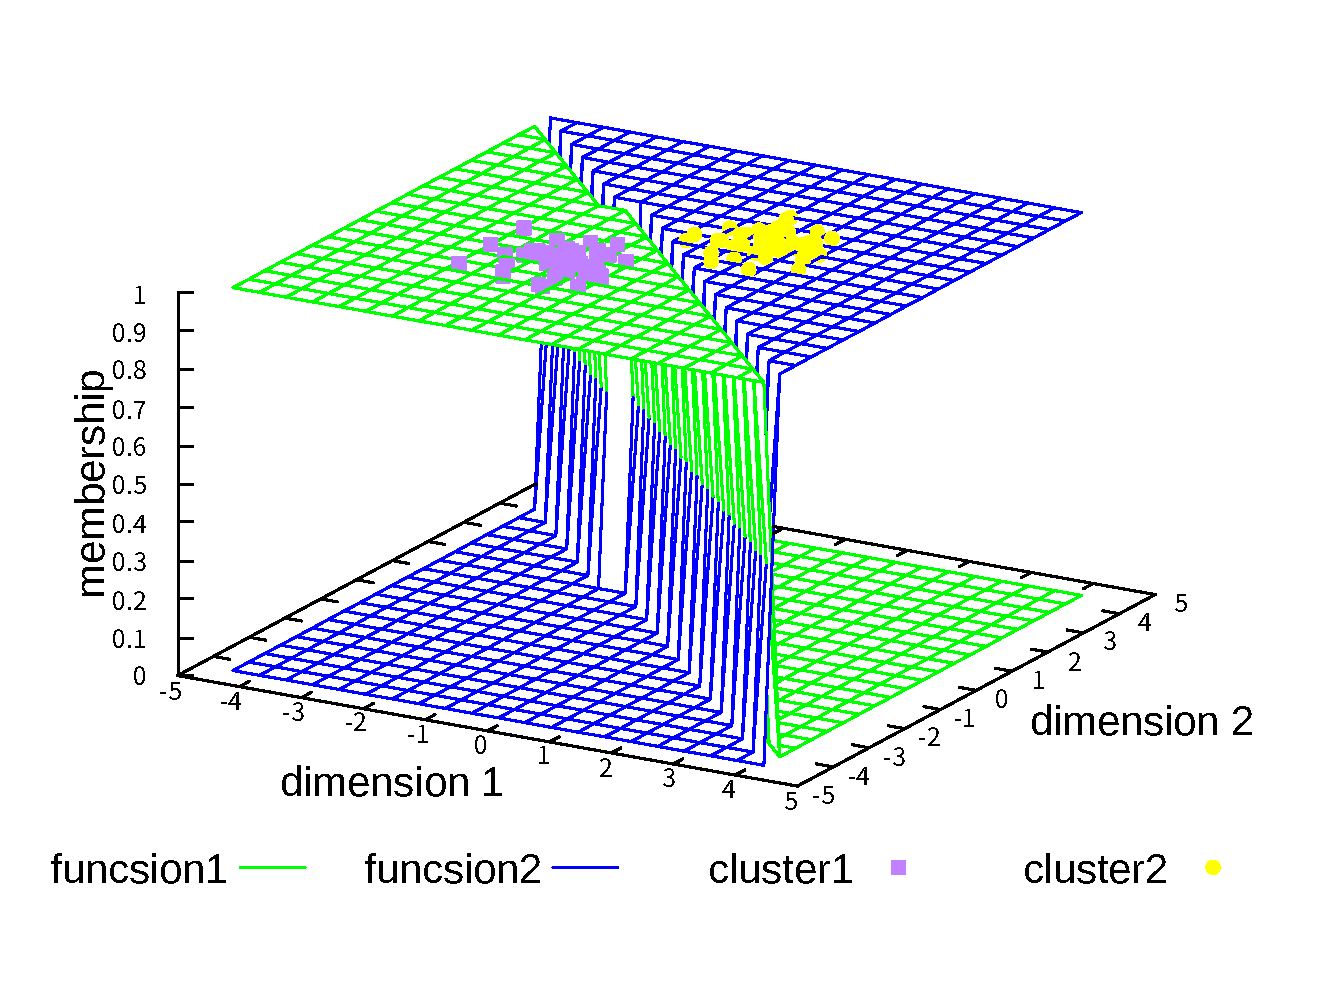
\includegraphics[width=40mm]{eFCMA-Lambda10000.pdf}
        \end{center}
        \captionsetup{labelformat=empty,labelsep=none}
        \caption{$\lambda=10000$}
        \label{fig:two}
      \end{minipage}
     \begin{minipage}{0.32\hsize}
        \begin{center}
          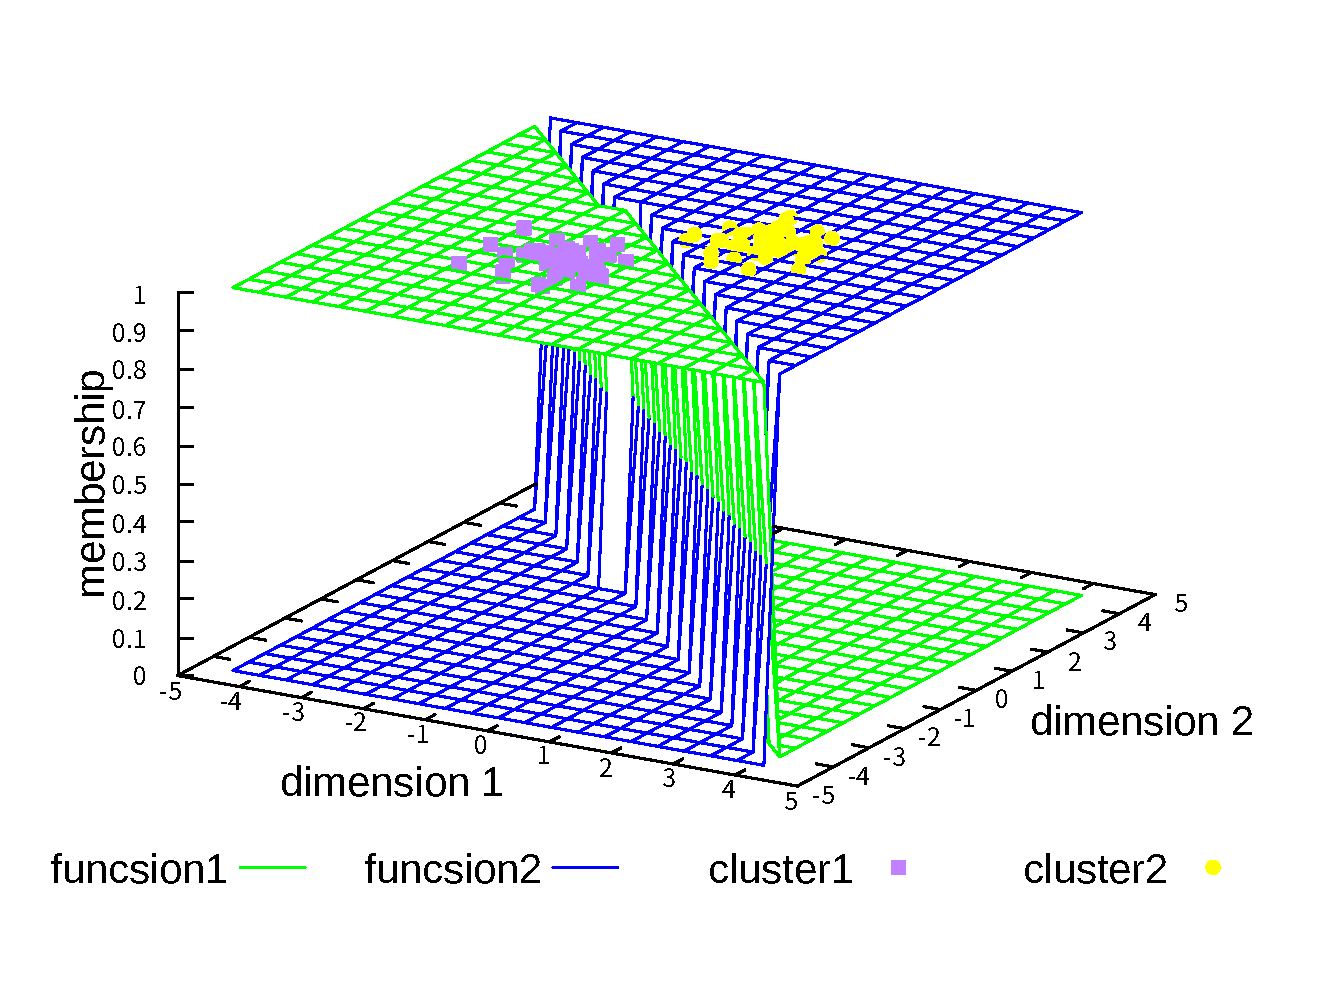
\includegraphics[width=40mm]{HCM.pdf}
        \end{center}
        \captionsetup{labelformat=empty,labelsep=none}
        \caption{HCM}
      \label{fig:three}
     \end{minipage}
    \end{figure}
  \end{block}
  \begin{block}{eFCMAの特徴}
    \begin{center}
      パラメータ$\lambda$を無限大に近づけるほどHCMに近づく
    \end{center}
  \end{block}
\end{frame}

\begin{frame}\frametitle{実験結果}
  \begin{block}{sFCMA}
    \begin{figure}[htbp]
      \begin{minipage}{0.32\hsize}
        \begin{center}
          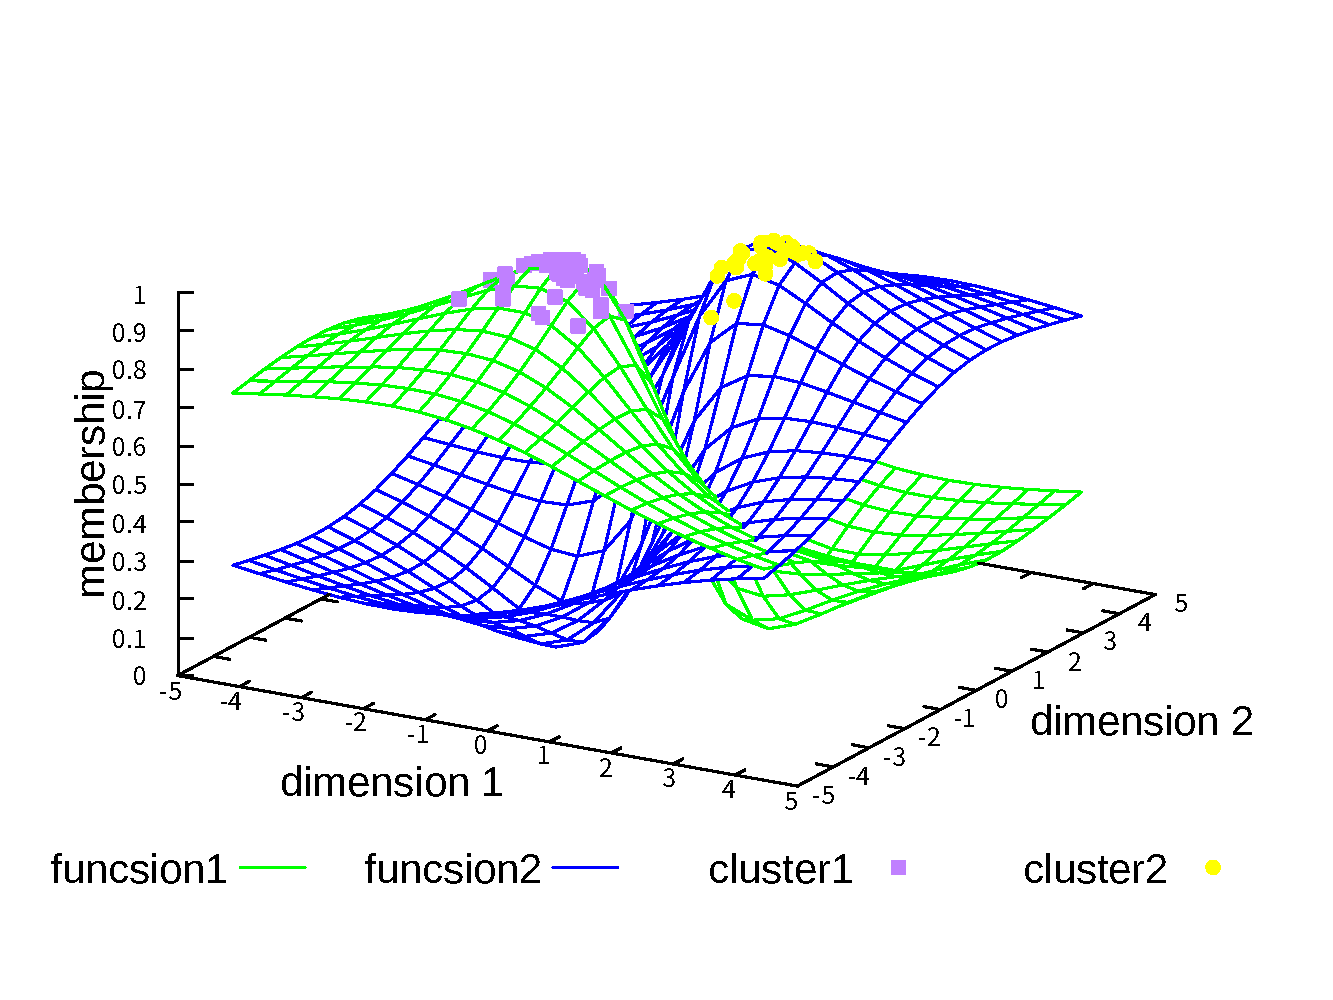
\includegraphics[width=40mm]{sFCMA-Em2.pdf}
        \end{center}
        \captionsetup{labelformat=empty,labelsep=none}
        \caption{$m=2$}
        \label{fig:one}
      \end{minipage}
      \begin{minipage}{0.32\hsize}
        \begin{center}
          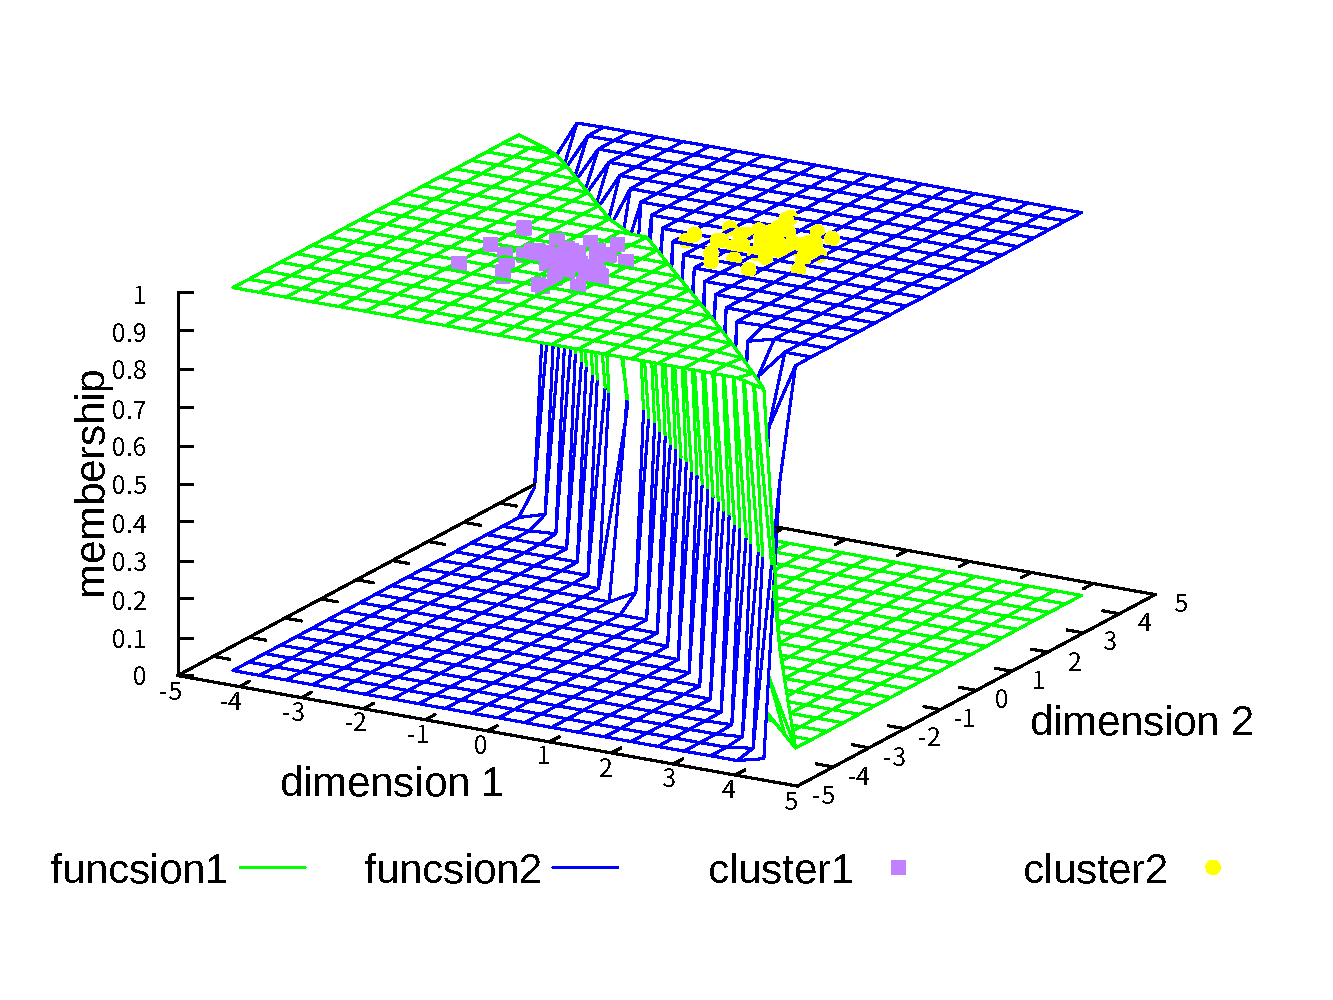
\includegraphics[width=40mm]{sFCMA-Em11.pdf}
        \end{center}
        \captionsetup{labelformat=empty,labelsep=none}
        \caption{$m=1.01$}
        \label{fig:two}
      \end{minipage}
     \begin{minipage}{0.32\hsize}
        \begin{center}
          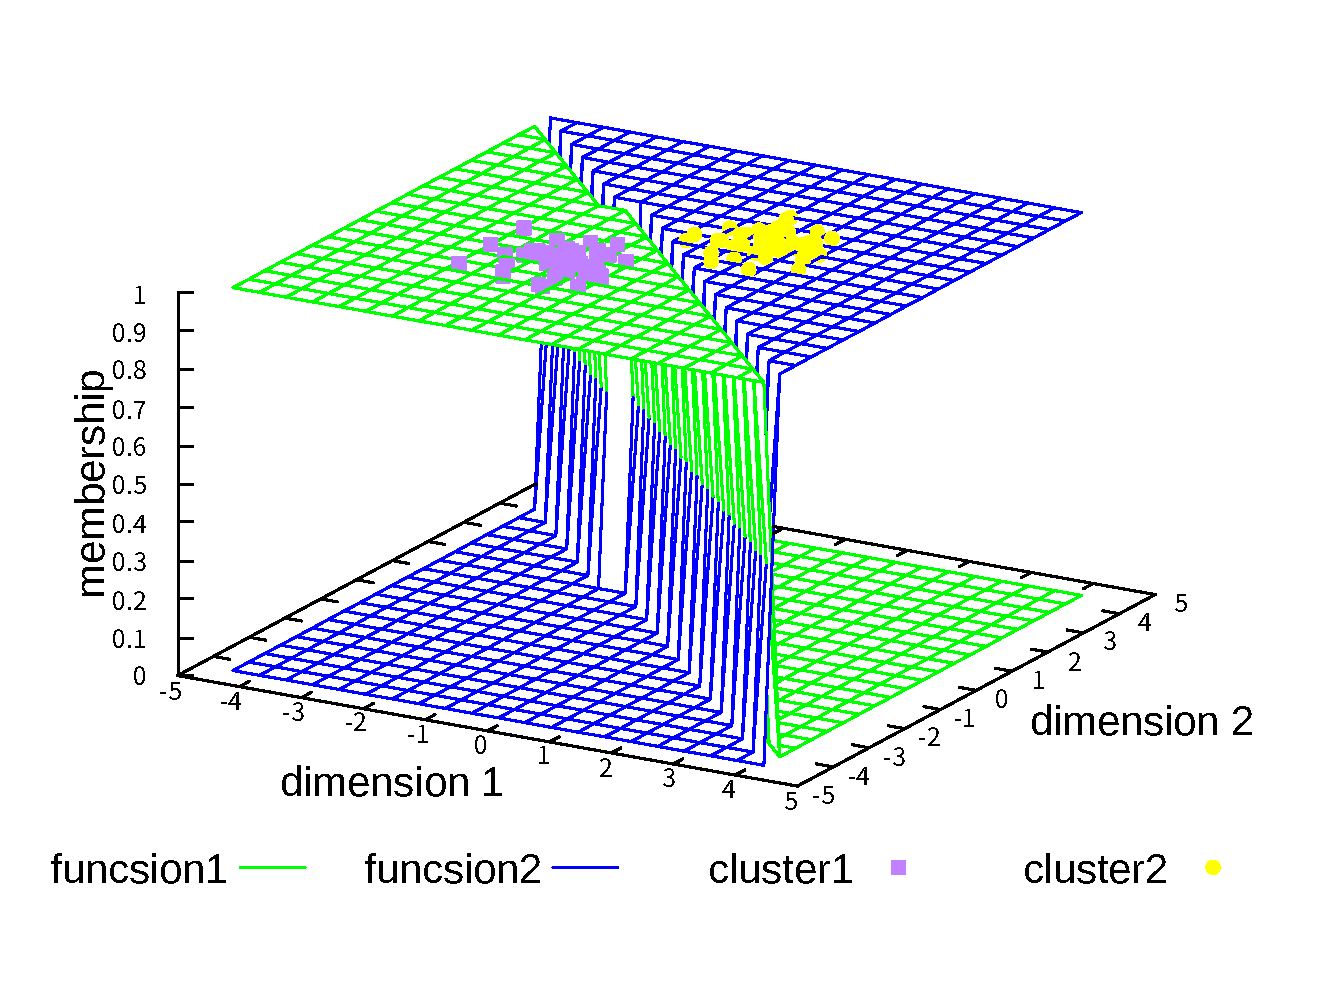
\includegraphics[width=40mm]{HCM.pdf}
        \end{center}
        \captionsetup{labelformat=empty,labelsep=none}
        \caption{HCM}
        \label{fig:three}
     \end{minipage}
    \end{figure}
  \end{block}
  \begin{block}{sFCMAの特徴}
    \begin{center}
      パラメータ$m$を1に近づけるほどHCMに近づく
    \end{center}
  \end{block}
\end{frame}

\begin{frame}\frametitle{実験結果}
  \begin{block}{qFCMA}
    %\vspace{5mm}
    \begin{figure}[htbp]
      \begin{minipage}{0.32\hsize}
        \begin{center}
          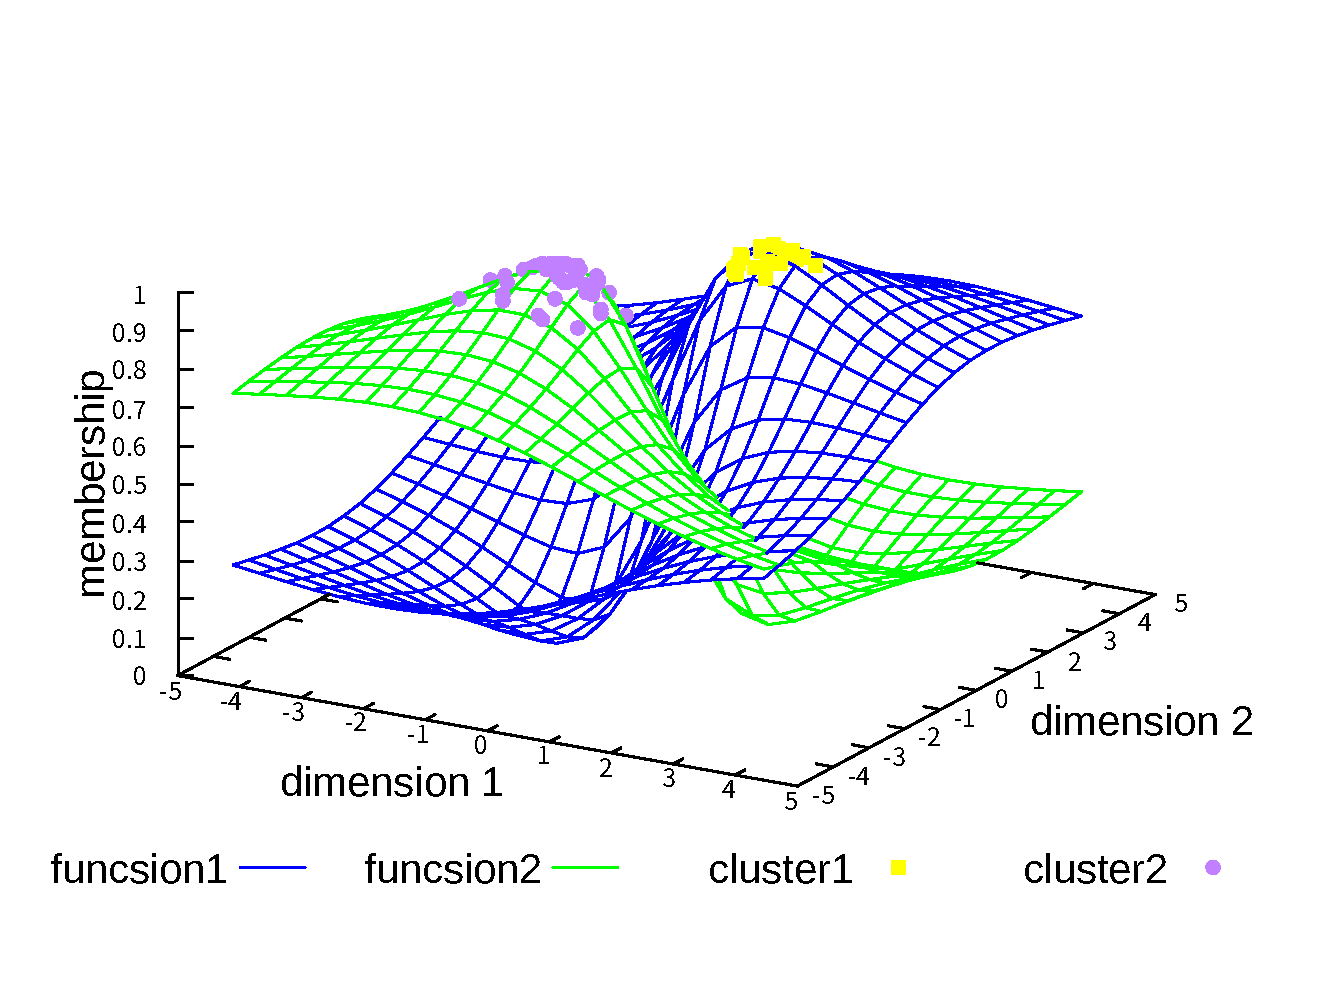
\includegraphics[width=40mm]{qFCMA-Em2-Lambda10.pdf}
        \end{center}
        \captionsetup{labelformat=empty,labelsep=none}
        \caption{$m=2.0$\;, \;$\lambda=10$}
        \label{fig:one}
      \end{minipage}
      %\hspace{1cm}
      \begin{minipage}{0.32\hsize}
        \begin{center}
          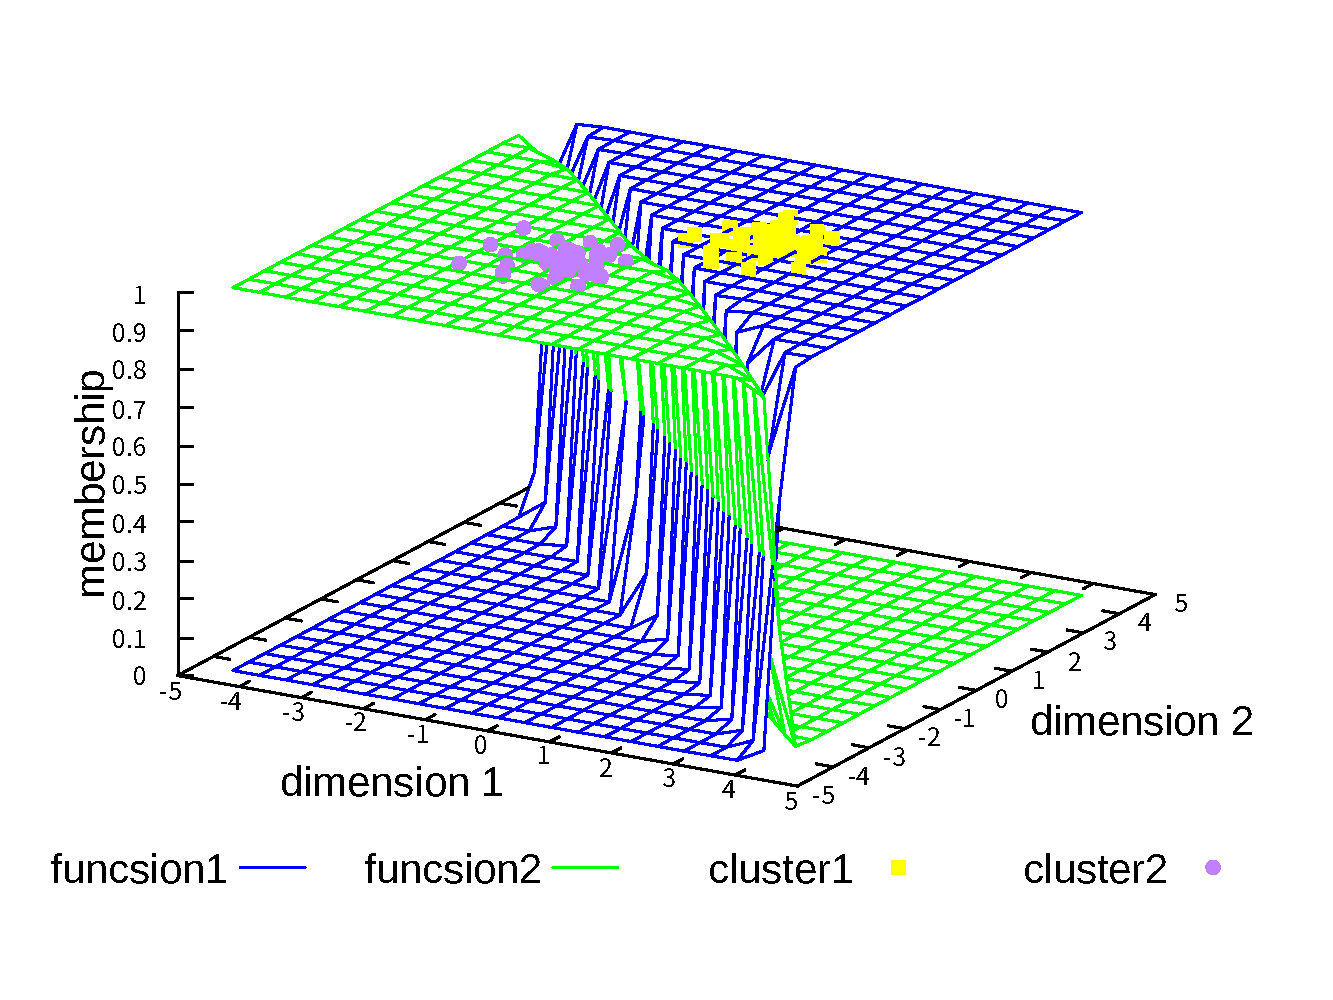
\includegraphics[width=40mm]{qFCMA-Em11-Lambda10.pdf}
        \end{center}
        \captionsetup{labelformat=empty,labelsep=none}
        \caption{$m=1.01$\;, \;$\lambda=10$}
        \label{fig:two}
      \end{minipage}
     \begin{minipage}{0.32\hsize}
      \begin{center}
       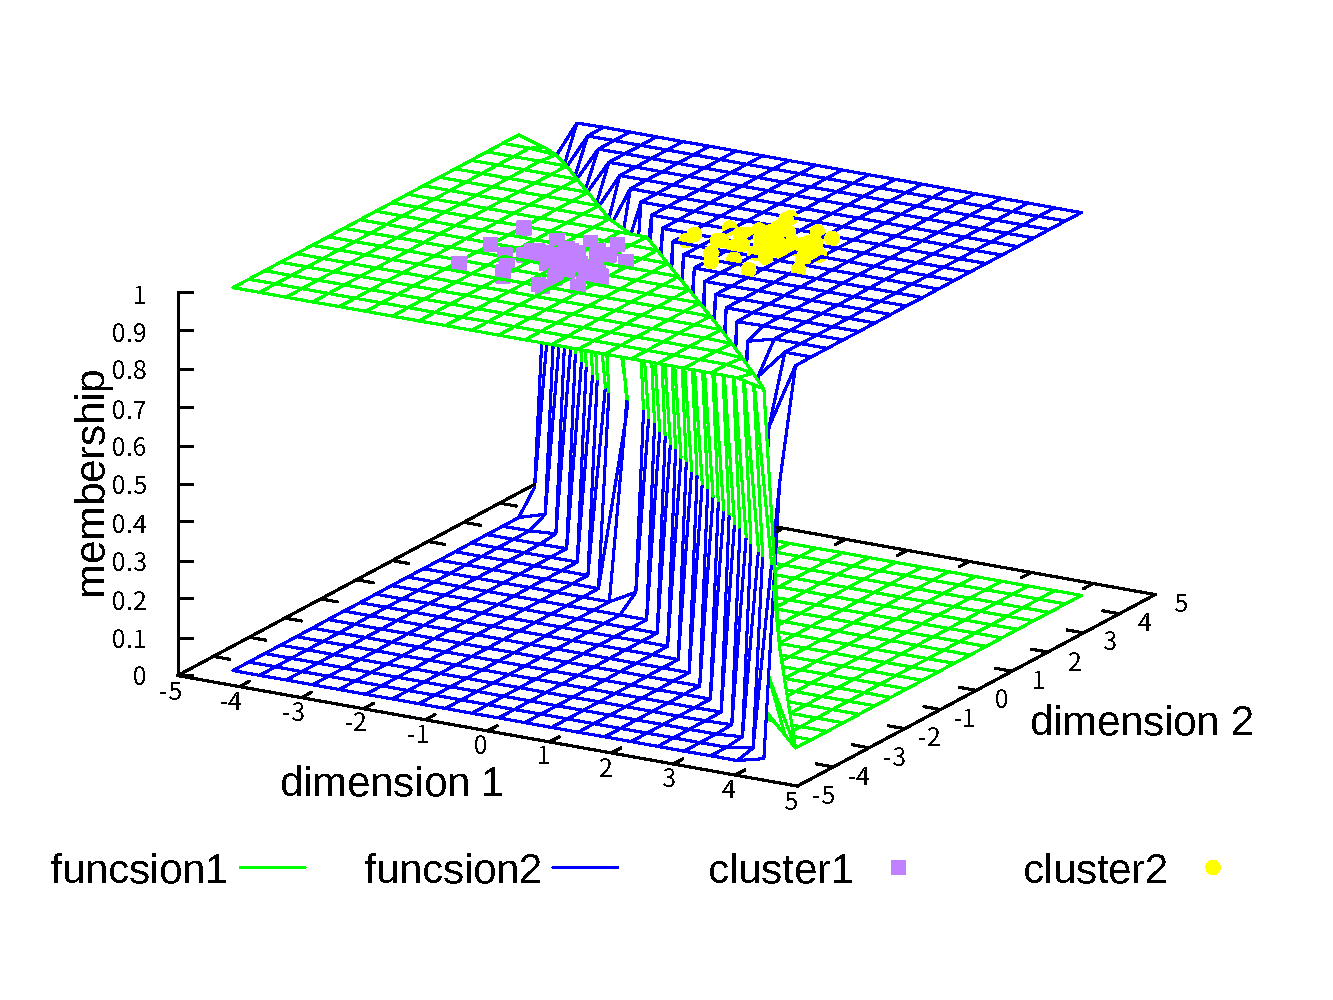
\includegraphics[width=40mm]{qFCMA-Em11-Lambda10000.pdf}
      \end{center}
      \captionsetup{labelformat=empty,labelsep=none}
      \caption{$m=1.01$\;, \;$\lambda=10000$}
      \label{fig:two}
     \end{minipage}
    \end{figure}
  \end{block}
  \begin{block}{qFCMAの特徴}
    \begin{itemize}
      \item パラメータ$\lambda$を無限大に近づけるとsFCMAに近づく
      \item パラメータ$m$を1に近づけるとeFCMAに近づく
    \end{itemize}
  \end{block}
\end{frame}

\begin{frame}\frametitle{各手法間の関係}
  \begin{center}
    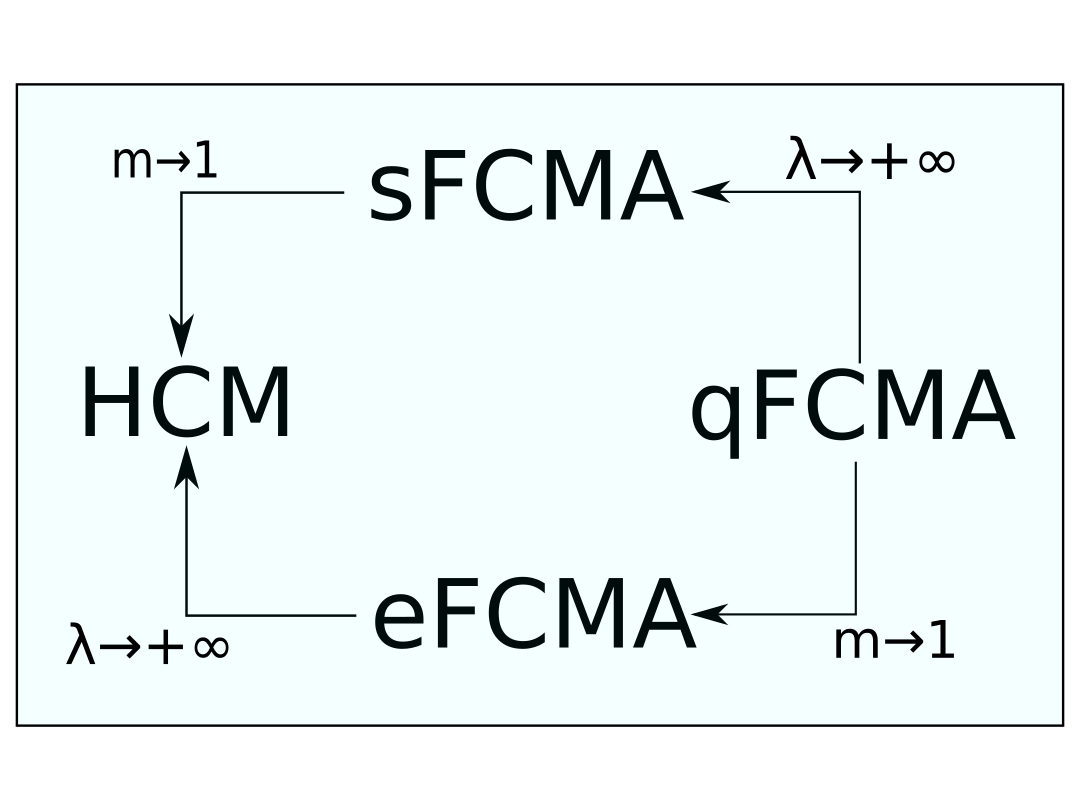
\includegraphics[height=60mm]{method.png}
  \end{center}
\end{frame}

\section{実データ実験}
\begin{frame}\frametitle{実データ実験}
  \begin{block}{使用する実データ}
    \begin{itemize}
     \item User Knowledge Modeling Data Set
     \item 被験者の勉強時間,試験結果など5属性を収録したデータ
     \item ソース : UCI  Machine Learning Repository
     \item 個体数 : 403
     \item クラス数 : 4(非常に低い,低い,中央,高い)
    \end{itemize}
  \end{block}
\end{frame}

\begin{frame}\frametitle{実験条件}
  \begin{block}{eFCMA}
    \begin{center}
      パラメータ$\lambda$を0.1から1刻みで100まで変化させる
    \end{center}
  \end{block}
  \begin{block}{qFCMA}
    \begin{itemize}
      \item パラメータ$\lambda$を0.1から1刻みで100まで変化させる
      \item パラメータ$m$を2から0.01刻みで1.01まで変化させる
    \end{itemize}
  \end{block}
  \begin{block}{sFCMA}
    \begin{center}
      パラメータ$m$を2から0.01刻みで1.01まで変化させる
    \end{center}
  \end{block}
\end{frame}

\begin{frame}\frametitle{アルゴリズム}
  \begin{enumerate}
  \item 正解帰属度を用いて帰属度を初期化する.
  \item 帰属度を用いてクラスタ中心及びクラスタサイズ調整変数を更新する.
  \item 収束すれば終了し,そうでない場合は$2$に戻る.
  \end{enumerate}
\end{frame}

\begin{frame}\frametitle{実験結果}
  \begin{block}{eFCMA}
    \begin{figure}[htbp]
      \begin{center}
        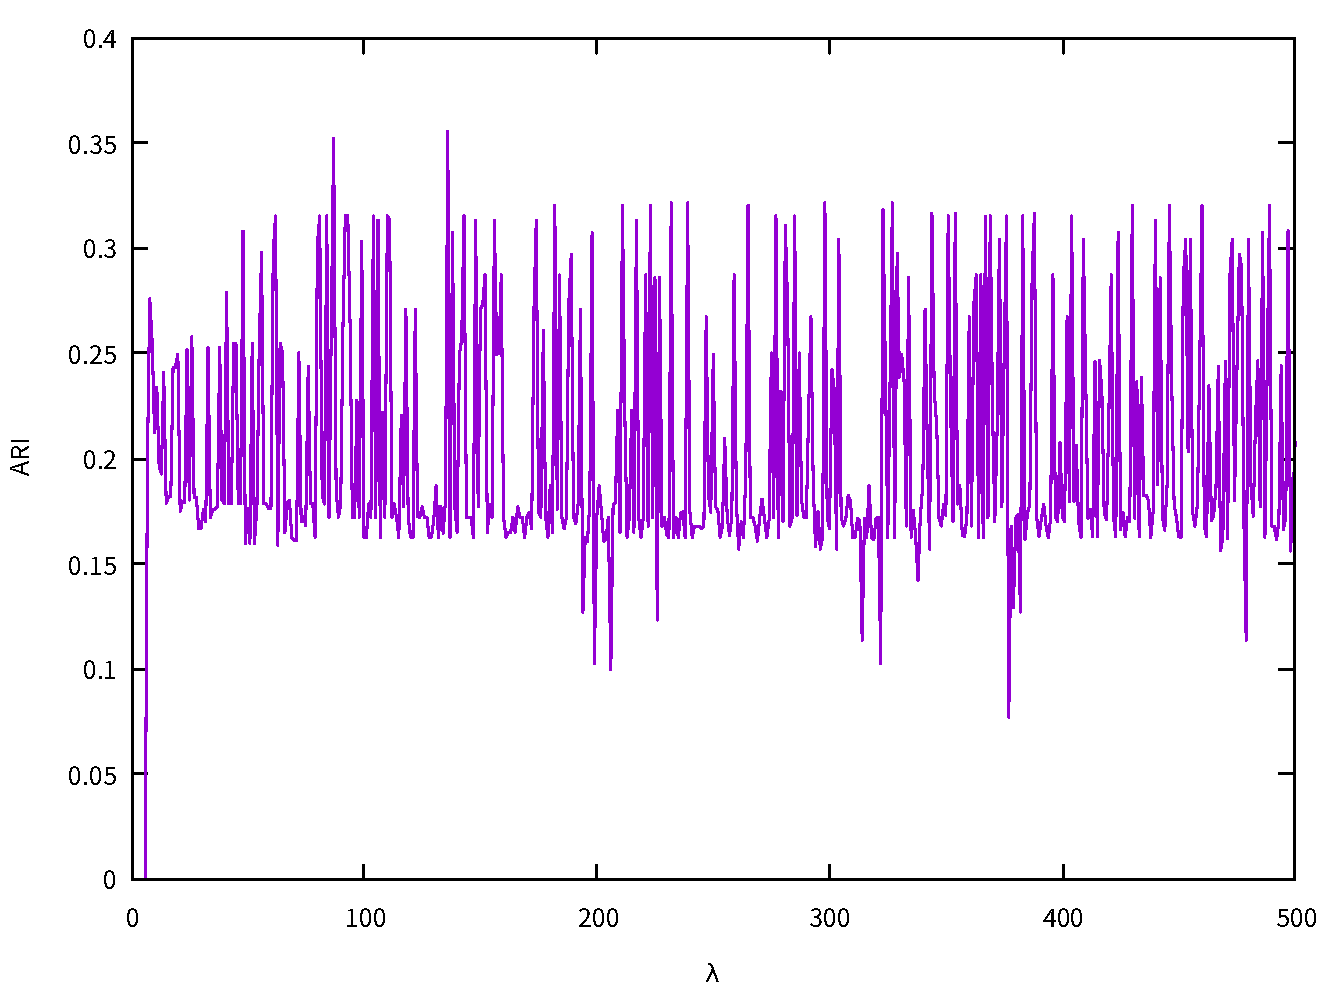
\includegraphics[height=60mm]{eFCMA_ARI.pdf}
      \end{center}
      \captionsetup{labelformat=empty,labelsep=none}
      \caption{最高ARI:0.352349 ($\lambda=67$)}
    \end{figure}
  \end{block}
\end{frame}

\begin{frame}\frametitle{実験結果}
  \begin{block}{sFCMA}
    \begin{figure}[htbp]
      \begin{center}
        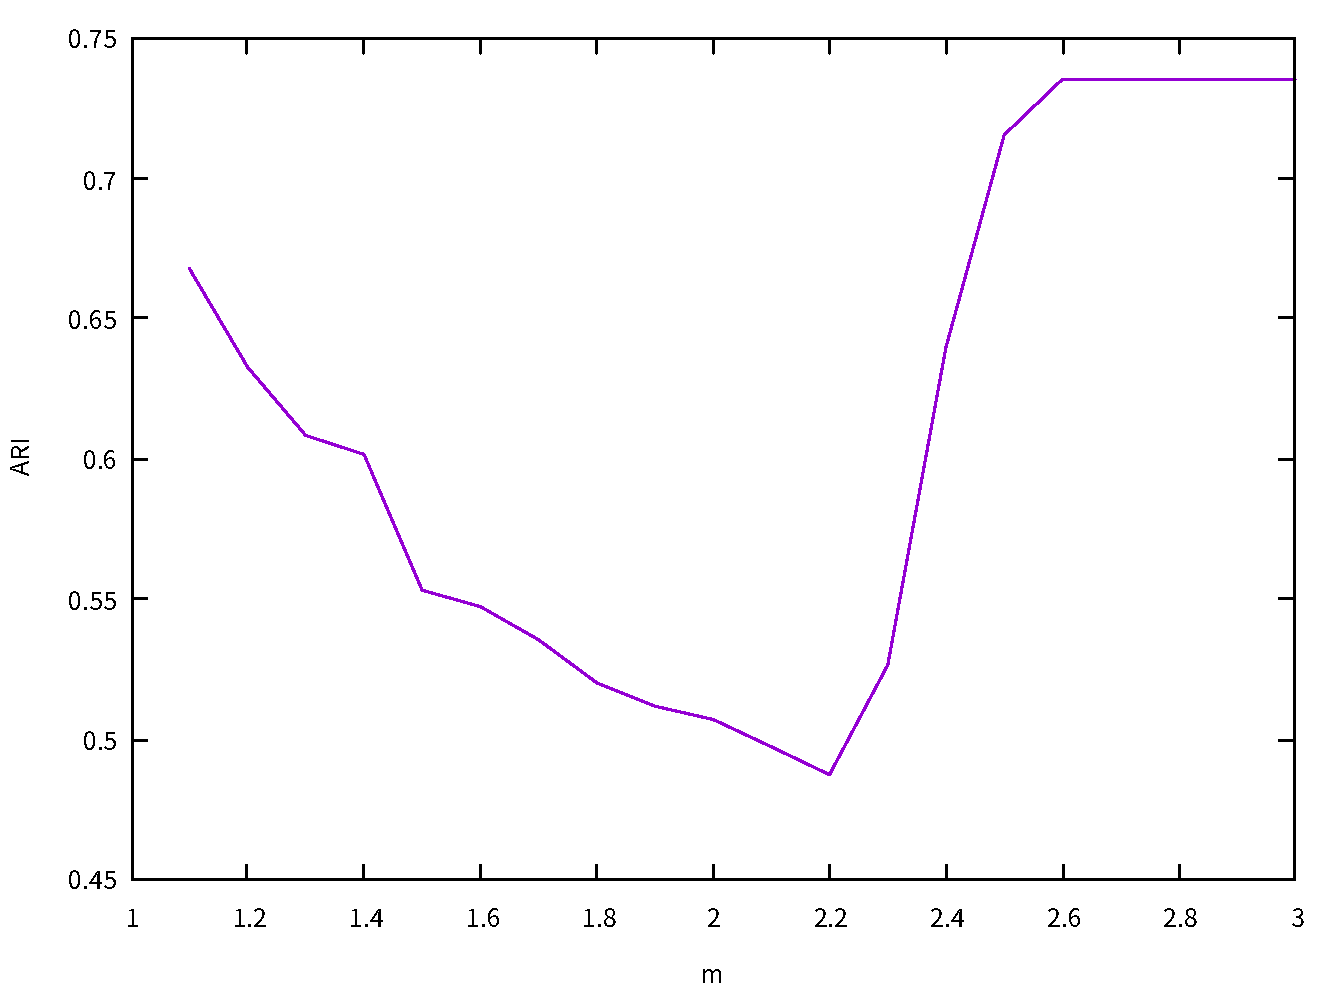
\includegraphics[height=60mm]{sFCMA_ARI.pdf}
      \end{center}
      \captionsetup{labelformat=empty,labelsep=none}
      \caption{最高ARI:0.715312 ($m=1.01$)}
    \end{figure}
  \end{block}
\end{frame}

\begin{frame}\frametitle{実験結果}
  \begin{block}{qFCMA}
    \begin{figure}[htbp]
      \begin{center}
        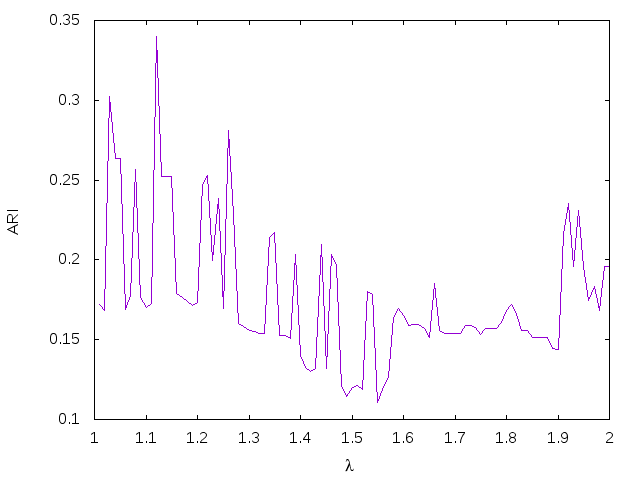
\includegraphics[height=60mm]{qfcma_ARI.png}
      \end{center}
      \captionsetup{labelformat=empty,labelsep=none}
      \caption{最高ARI:0.339808 ($\lambda=99$, $m=1.12$)}
    \end{figure}
  \end{block}
\end{frame}

\begin{frame}\frametitle{実験結果}
  \begin{block}{各手法の最高ARI}
    \vspace{5mm}
    \begin{table}
      \begin{tabular}{ l || c | c }\hline
        eFCMA & 0.352349 & $\lambda = 67$\\ \hline  
        sFCMA & 0.715312 & $m = 1.01$\\ \hline
       qFCMA & 0.339808 & $\lambda = 99 $\;, \;$m = 1.12$\\  \hline
      \end{tabular}
    \end{table}
  \end{block}
  \begin{block}{評価}
    \begin{center}
      sFCMAが最も高評価
    \end{center}
  \end{block}
\end{frame}

\section{考察}
\begin{frame}\frametitle{考察}
  \begin{block}{考察}
    \begin{itemize}
    \item sFCMAとeFCMA及びqFCMAとの差は,エントロピー項の有無.
    \item エントロピー項を削除したことが計算結果に影響したと考えられる.
    \end{itemize}
  \end{block}
\end{frame}

\section{まとめ}
\begin{frame}\frametitle{まとめ}
  \begin{block}{背景}
   \begin{center}
    データ量の増大によりクラスタリングに注目が集まっている
   \end{center}
  \end{block}
 \begin{block}{目的}
  \begin{center}
   クラスタサイズ調整変数を導入した手法の中で有用なものを発見する
  \end{center}
 \end{block}
  \begin{block}{実験結果}
   \begin{center}
    sFCMAが最も高評価となった
   \end{center}
  \end{block}
 \begin{block}{考察}
  \begin{center}
   エントロピー項を削除したことが計算結果に影響したと考えられる
  \end{center}
 \end{block}
\end{frame}

\section{補足}
\begin{frame}\frametitle{クラスタリングについて}
  \begin{block}{クラスタリングとは}
   \begin{center}
   データを類似度に基づいてグループ化するデータ分析手法の1つ
   \end{center}
  \end{block}
  \vspace{5mm}
  \begin{figure}[htbp]
    \begin{minipage}{0.4\hsize}
      \begin{center}
        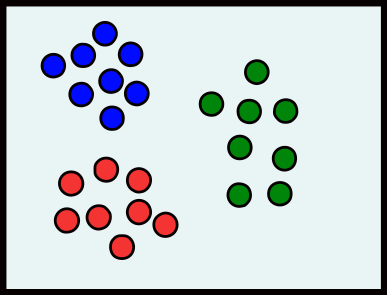
\includegraphics[width=40mm]{before_clustering.png}
      \end{center}
      \captionsetup{labelformat=empty,labelsep=none}
      \caption{クラスタリング前}
      \label{fig:one}
    \end{minipage}
    \hspace{1cm}
    \begin{minipage}{0.4\hsize}
      \begin{center}
        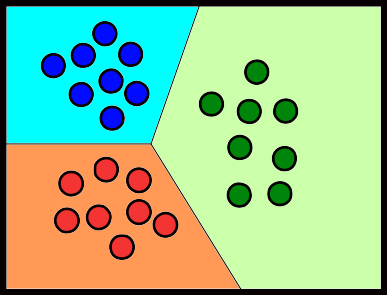
\includegraphics[width=40mm]{after_clustering.png}
      \end{center}
      \captionsetup{labelformat=empty,labelsep=none}
      \caption{クラスタリング後}
      \label{fig:two}
    \end{minipage}
  \end{figure}
\end{frame}

\begin{frame}\frametitle{HCM\scriptsize(Hard $c$-means)}
  \begin{block}{最適化問題}
    $\underset{u,v}{\text{minimize}}$
    $\sum_{i=1}^C\sum_{k=1}^Nu_{i,k}||x_k-v_i||_2^2\quad$ subject
    $\;$ to $\; \sum_{i=1}^Cu_{i,k}$=1 \;and\; $u_{i,k}\in\{0,1\}$
  \end{block}
  \begin{align*}
    u_{i,k}&=\begin{cases}
    1 & (i=\text{arg min}_{1 \leq j \leq C}\{||x_k-v_i||_2^2\}) \\
    0 & (\text{otherwise})
    \end{cases},\\
    v_{i}&=
    \frac{\sum_{k=1}^N u_{i,k}x_{k}}{\sum_{k=1}^N u_{i,k}}.
  \end{align*}
\end{frame}

\begin{frame}\frametitle{eFCMAの更新式}
  \begin{eqnarray*}
    &v_{i}& =\frac{\sum_{k=1}^Nu_{i,k}x_{k}}{\quad\sum_{k=1}^Nu_{i,k}},\\
    &u_{i,k}&=\frac{\pi_{i}\exp(-\lambda||x_k-v_i||_2^2)}{\sum_{j=1}^C\alpha_{j}\exp(-\lambda||x_k-v_j||_2^2)},\\
    &\alpha_{i}&=\frac{\sum_{k=1}^Nu_{i,k}}{\quad N}.\\
  \end{eqnarray*}
\end{frame}

\begin{frame}\frametitle{qFCMAの更新式}
  \begin{eqnarray*}
    &v_{i}&=\frac{\sum_{k=1}^N(u_{i,k})^mx_{k}}{\quad\sum_{k=1}^N(u_{i,k})^{m}},\quad\\
    &u_{i,k}&=\frac{\alpha_{i}(1+\lambda(1-m)||x_i-v_k||_2^2)^\frac{1}{1-m}}{\quad\sum_{j=1}^C\alpha_{j}(1+\lambda(1-m)||x_j-v_k||_2^2)^\frac{1}{1-m}},\\
    & \alpha_{i}&=\frac{1}{\sum_{j=1}^C\left(\sum_{k=1}^N\frac{(u_{j,k})^m(1-\lambda(1-m)d_{j,k})}{(u_i,k)^m(1-\lambda(1-m)d_{i,k})}\right)^{\frac{1}{m}}}.\\
  \end{eqnarray*}
\end{frame}

\begin{frame}\frametitle{sFCMAの更新式}
  \begin{eqnarray*}
    &v_{i}&=\frac{\sum_{k=1}^N(u_{i,k})^mx_{k}}{\quad\sum_{k=1}^N(u_{i,k})^{m}},\\
    &u_{i,k}&=\frac{1}{\sum_{j=1}^c\frac{\alpha_{j}}{\alpha_{i}}\left(\frac{d_{j,k}}{d_{i,k}}\right)^\frac{1}{1-m}},\\
    &\alpha_{i}&=\frac{1}{\sum_{j=1}^C\left(\sum_{k=1}^N\frac{(u_{j,k})^md_{j,k}}{(u_{i,k})^md_{i,k}}\right)^{\frac{1}{m}}}.\\
  \end{eqnarray*}
\end{frame}

\end{document}
